\documentclass{article}
\usepackage{amsmath}
\usepackage{graphicx}
\usepackage{wrapfig}

% Layout
\usepackage{amssymb}
% Margins
\topmargin=-0.75in
\evensidemargin=0.0in
\oddsidemargin=-0.5in
\hoffset=1.0in
\textwidth=5.5in
\textheight=9.0in
\headsep=0.25in

\usepackage[
backend=biber, 
natbib=true,
style=numeric,
sorting=none
]{biblatex}


%----------------------------------------------------------------------------------------
%	TITLE SECTION
%----------------------------------------------------------------------------------------

\newcommand{\horrule}[1]{\rule{\linewidth}{#1}} % Create horizontal rule command with 1 argument of height

%----------------------------------------------------------------------------------------
%	REFERENCES
\addbibresource{Report.bib}
\bibliography{Report.bib}

%----------------------------------------------------------------------------------------

\title{	
\normalfont \normalsize 
\textsc{American University of Armenia} \\ [25pt] % Your university, school and/or department name(s)
\horrule{0.5pt} \\[0.4cm] % Thin top horizontal rule
\huge Searching the Quoridor\\ % The assignment title
\horrule{2pt} \\[0.5cm] % Thick bottom horizontal rule
}

\author{
	Petros Tepoyan \\
	Samvel Topuzyan \\
	Alexander Israyelyan } % Your name

\date{\normalsize\today} % Today's date or a custom date

\begin{document}

\maketitle

\section*{Abstract} \indent

	This paper analyses different approaches to implementing searching strategies for a board game Quoridor. It explores the application of Monte Carlo Tree Search (MCTS), minimax with alpha-beta pruning, and expectimax algorithms, focusing on their ability to navigate the game's complex state space. The goal is to demonstrate how AI can adeptly handle Quoridor's intricate rules and large branching factor, contributing to advanced AI techniques in board game strategy.


\tableofcontents

\section{Introduction $|$ Game Rules } \indent

	\begin{wrapfigure}{r}{0.25\textwidth} %this figure will be at the right
	    \centering
	    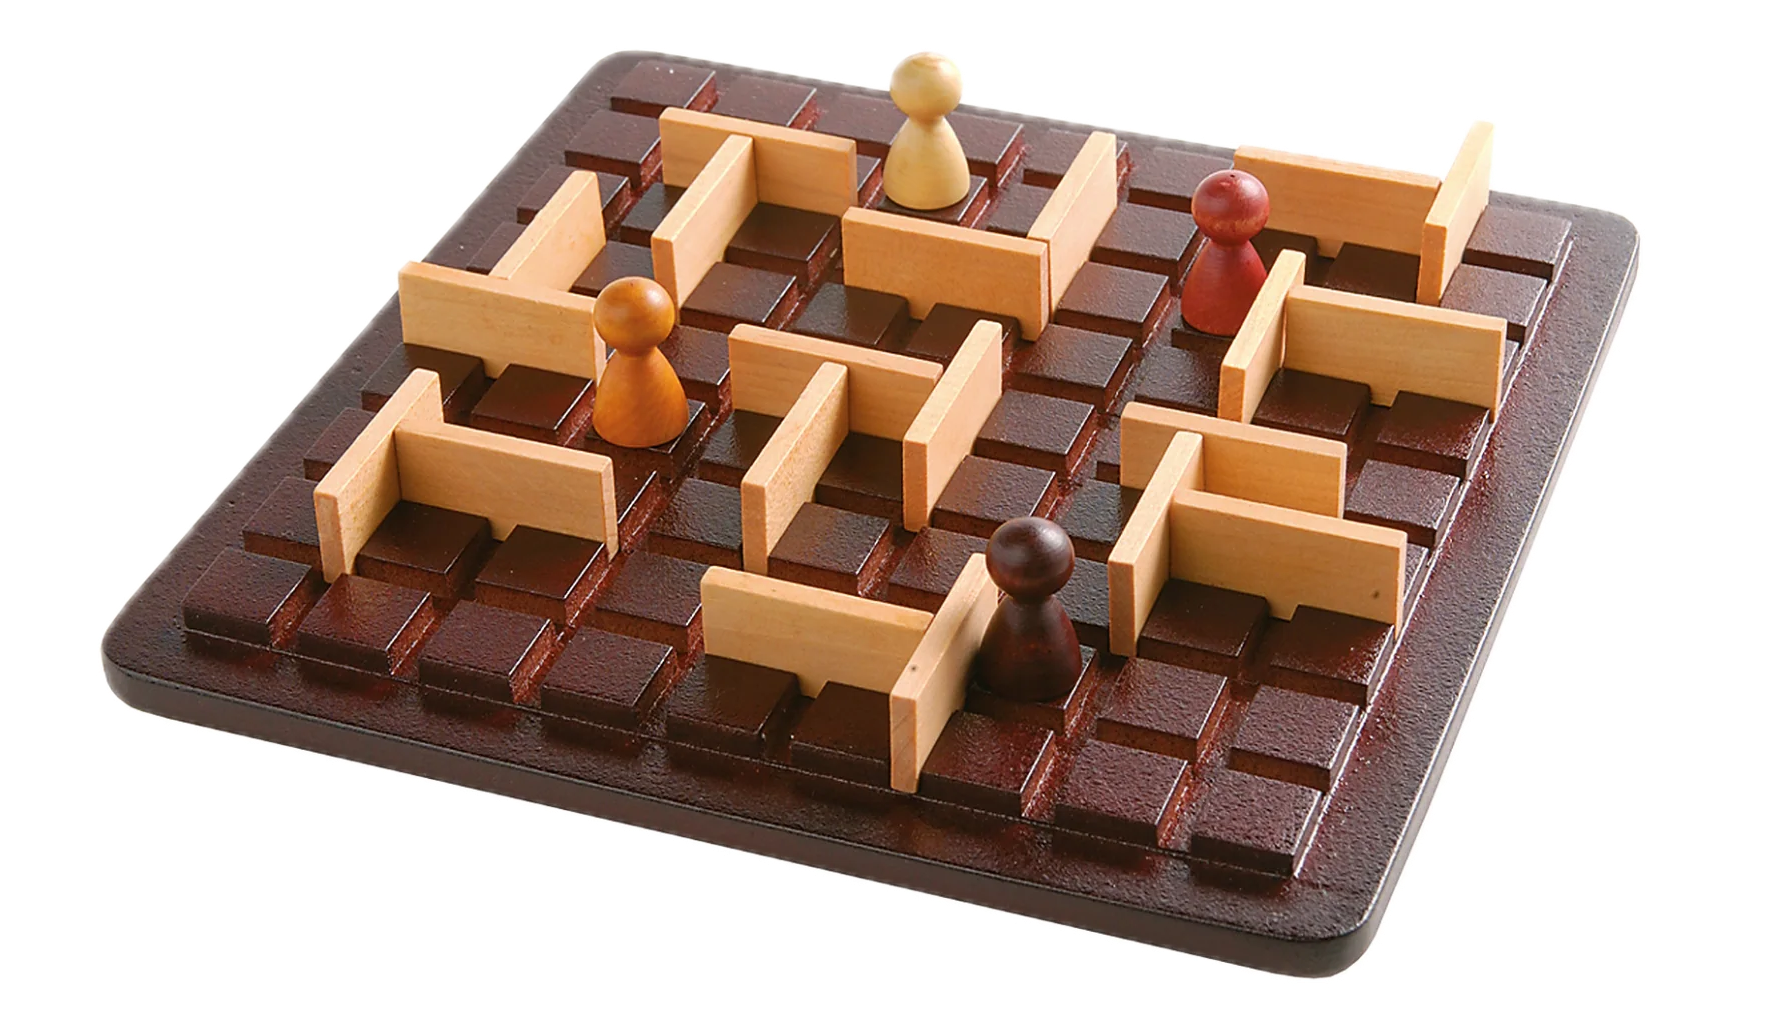
\includegraphics[width=0.25\textwidth]{game}
	\end{wrapfigure}

	Quoridor is a two- or four-player strategy game designed by Mirko Marchesi and published by Gigamic Games \cite{Wikipedia_Quoridor}. It is played on a 9x9 game board. Each player is represented by a pawn. In two-player case the pawns are placed at the first and the last rows, in the center column. In the four-player case, the two additional pawns are placed at the first and the last columns, in the center row. The objective of each player (both in two-player and four-player scenarios) is to be the first to get to the opposite edge of the board. \cite{ai_agent} 
	
	The icing on the cake of this game is the twenty walls, each player has ten or five, depending on whether there are two or four players. These walls are flat and are twice the length of a square. They can be placed on the border which runs in between the squares. Walls cannot overlap or have a part that is outside of the board. They block the path of all pawns, which must bypass them. The walls are stationary after they are deployed and cannot be removed or displaced. Furthermore, a wall cannot be placed, if after that any player does not have a path to goal state.
	
	The game is played in turns, the players perform an action one after another, in a circular queue manner. At each turn a player’s action may be either to move to an adjacent square, or to place a wall on any free and valid place on the board. An adjacent square is either the immediate neighboring square to the North, or to the East, or to the South, or to the West. If at any step, there is another player in an adjacent square, the player may jump over this square. If the jump cannot be made (off the edge of the board), any other direction is accessible. 

\section{Literature review}

\subsection{Monte Carlo Tree Search for Quoridor} \indent

In their paper Victor Massagu´e Respall, Joseph Alexander Brown and Hamna Aslam conduct a preliminary study of Quoridor, using Monte Carlo Tree Search (MCTS) \cite{monte_carlo}. They claim that their system performs well against existing methods at the time of writing it. It is said to beat implementations using genetic algorithms. They chose MCTS to address issues connected with large space-complexity, large branching factor and difficulties to evaluate the state of the game in the middle. Final states of game are evaluated using Upper Confidence Bound applied to trees. This allows to generate more accurate values when the tree grows larger. They also use rollouts in the MCTS, the average of which can provide an effective position evaluation, achieving accurate performance. 

One of the reasons they use MCTS is that it is based on random sampling of game states and does not rely on brute force, which can be rather problematic considering this immense size of the state space. They keep count of how many times a node was selected and use it alongside with a win score to evaluate the current state of the board. The algorithm consists of 4 phases: Selection, Expansion, Simulation, Backpropogation. Selection includes starting with a root node and selecting a child node with maximum win rate. To maximize the fairness of the child selection process, the algorithm uses Upper Confidence Bound applied to Trees (UCT). During expansion game tree is expanded, by generating all possible states from the leaf node, when UCT can no longer be applied. For Simulation, a node is randomly chosen after the expansion and the game is simulated to the end for both players. Backpropagation updates the nodes based on simulation results. These 4 phases are repeatedly looped for a fixed number of times. 

The project uses Java implementation of this algorithm. A problem they ran into was that after just only 5000 simulations the program runs out of memory, because MCTS generates too many nodes. They solve it by storing only the move to be performed and the scores of the node, instead of saving the whole board in each generated node. Several agents are represented in the project: 120k and 60k simulation agents, where 120k and 60k are the numbers of rollouts per move. These are developed by the authors. For comparison, they use an alternative agent with 4 increasing levels and a genetic algorithm agent. In the end they conclude that the 60k agent performed better than 120k agent, with 	a smaller runtime. They conclude that the heuristic they used can be improved to decide better quality moves and taking into account more features, such as the number of fences used, could improve the efficiency.


\subsection{Minimax, Alpha-Beta Pruning, Expectimax for Quoridor} \indent

In 2021, Dimitrije Karanfilović published a Python implementation of Quoridor AI that uses minimax (with or without alpha-beta pruning), expectimax, and MCTS adversarial searches \cite{python_but_worse}.

For minimax, a specific state evaluation function was used that is tailored for Quoridor experience. To estimate shortests paths to victory, the function summons A*-search with a simple path-finding heuristic that just returns the horizontal perpendicular distance from current position to the opposite side of the board, multiplied by a suitable factor. Then, the evaluation function returns an assessment of the current game state according to multiple negative and positive factors to enable the minimax algorithm. For instance, the favorability of the situation is increased by the opponent’s perpendicular distance and the player’s shortest-path distance to their goal, as well as the difference between each player’s remaining walls; it is equivalently decreased by opponent’s shortest-path distance and the player’s perpendicular distance to the goal. Additionally, the evaluation function penalizes moves where shortest-path A*-star computation failed, and encourages moves that end up in terminal, win states. 

If alpha-beta pruning version for minimax is selected, a track of alpha and beta is kept in order to discard child nodes that couldn’t possibly affect the final decision.

For expectimax, the opponent has chance nodes, since their strategy in this implementation is not always known. The utility function value for chance nodes is computed by averaging child nodes. 

\subsection{Retrograde Analysis of Quoridor} \indent

In 2023, Mr.Takuro Iwanaga and Satoshi Ikeda released a paper, where they reused the results of the reduced version of the game Quoridor to draw some interesting conclusions \cite{retrograde}. This method is called “Retrograde analysis” and in the first place lists all the legal positions, after it does a search to find the most optimal move, doing backwards analysis starting from the final positions to the initial position. Retrograde analysis is useful when the same state repeats during the course of the game, but requires a substantial amount of memory. They have conducted several experiments, during which, they start with a 5x5 board for the first experiment, and gradually increase the size of dimensions of board, but only using odd numbers for board dimensions. As their research suggests, the game is biased in favor of the player one when there is an odd number of fences, and when there is an even number of fences, the game is biased in favor of the player two.

\subsection{AI for Quoridor in Javascript.} \indent

	In this project Kyutae Lee implements yet another AI for the game Quoridor. In his Github repo he refers to 3 previous works which, in some way, had influence over his work \cite{javascript}. About the first one we already talked about: it is our first work reviewed - “Monte Carlo Tree Search for Quoridor”. This work led Kyutae to use MCTS in his agent. The second one is Daniel Borowski's Quoridor AI, where he uses minimax of depth ~2. The third one is Martijn van Steenbergen's SmartBrain 4. Here the negamax algorithm is used with depth of 4. In this project there are also SmartBrain1, SmartBrain2 and SmartBrain3 with depths of 1, 2, 3 correspondingly, but the strongest is SmartBrain4 with depth of 4. 
	
	Some of the heuristics he used in the latest v0.3 agent are available. The branching factor in this game is rather large, considering the large number of possible actions to do in a state. However, some actions are kind of equivalent to each other in a sense that logically they result in similar states, which do not change the game balance much. To decrease the branching factor, Kyutae uses a notion of “probable” actions. “Probable” next walls are the followings: 
	\begin{itemize}
		\item Walls near the pawns (to complicate the opponent’s job or help your pawn)
		\item Walls near already positioned walls
		\item Horizontal walls in the far left or far right
	\end{itemize}
	
	During the MSTC rollout phase he uses a constant probability of $A=0.7$ for choosing an action to move the pawn, and $1-A$ to choose action of placing a wall. If the agent has no walls left, that state is penalized. 
	
	During the selection/expansion phase of MSTC, in case there are no walls at the opponent's disposal, the pawn is moved only in the direction of the shortest path, and places walls only to disrupt the opponent’s pawns. This heuristic comes handy at the end of the game to decrease the branching factor. 
	
	Also, some common openings are considered during the first few states of the game.
	
	Results and efficiency comparisons between this and other AI agents are available. Martijn's SmartBrain 4 may seem stronger than Daniel's Quoridor AI, but the latter somehow managed to exhaust the walls of Kyutae’s 60k v0.2 agent quickly and lose the game. The v0.3 60k agent performs better than its predecessor and won 67 out of 100 games. And, in general, performed better against the other agents, than the 60k v0.2 agent.

\subsection{Python Quoridor AI}
\subsubsection{How the Problem is Solved}

In this project, Alain Rinder approached the problem with best caution \cite{closest_impl}. He did not present search strategies we are aiming to incorporate, but nicely designed the architecture of the game itself. Also, he implemented the game itself, which we may borrow in the future if we manage to do so. Here are some findings from investigating his solution:


\begin{enumerate}
	\item \textbf{Classes and Inheritance:} The code uses a class-based approach, with classes like `Game`, `Board`, `Pawn`, `Fence`, etc., representing different game elements. This object-oriented design is suitable for such simulations. However, they do not use proper OOP, because `Fence` and `Pawn` know how to place themselves on the board, how to move and they have a reference to the board, which is not a good practice.
	\item \textbf{Modular Design:} The code is split into different files and classes (`Game.py`, `GridCoordinates.py`, etc.), each handling specific aspects of the game. This makes the code more organized and maintainable. Speaking of the abstraction over coordinates (`GridCoordinates`), it is a good idea to borrow, because we can simplify access to left/right/up/down tiles. 
	\item \textbf{Game Logic and Rules:} The `Game` class manages the game rounds and player turns, while the `Board` class handles the game grid, including valid moves and placements for pawns and fences. One of the flaws that can be seen here is that `Board` class just “knows” too much. A better approach would be to split up responsibilities and use services inside the `Board` class to implement better readability and bug-less code.
	\item \textbf{Moves:} They do not return all the moves and then try to get the filter out valid ones. Instead, they check for valid moves right away. This gives a great boost in performance.
	\item \textbf{Path Finding:} They have solved the problem of obscured path by using Breadth First Search. Although it sounds like a brute-force solution, that is the most optimal in the sense of implementation time. If it works, it is good enough. We may try A*, but for that we need to come up with a good heuristic. 
	\item \textbf{No Search Implementation:} They do not implement any search techniques to find better moves. They use Breadth First Search to detect obscured paths, but that is it. For Bot Players they use other techniques. 
	\item \textbf{Players:} They have multiple types of bots, which we can adopt:
	\begin{enumerate}
		\item Build and run - places a fence and moves forward if possible
		\item Runner bot - only goes forward wherever possible
		\item Builder - places fences till does not have any, and start moving forward
	\end{enumerate}
   
\end{enumerate}

\subsubsection{Drawbacks of their solution}
\begin{enumerate}
	\item \textbf{Complexity}: The code is quite extensive and could be overwhelming for new developers or those unfamiliar with Python's class-based structure.
	\item \textbf{Potential for Redundant Calculations}: The game recalculates valid moves and fence placements frequently, which might be inefficient.
	\item \textbf{Limited Scalability}: The game seems to be designed primarily for a specific set of rules and might require significant rework for different game types or additional features.
	\item \textbf{Error Handling}: The code lacks comprehensive error handling and logging, which is crucial for debugging and user experience.

\end{enumerate}
Although this implementation has many flaws, they have solved the problem, and solved it with interesting solutions. It is worth borrowing some of their ideas for future development of our project. 

\section{Future Plans:}

Here are some important notes:
\begin{enumerate}
	\item We are going to use Alpha-Beta and Minimax search strategies. They are suitable for games and relatively easy to implement. If we have time, we will try to implement other informed search strategies like A* and Dejkstra.
	
	\item To simplify the game, we are not going to include the case when the game is played by 4 players, that would just multiple the number of calculations in already complex game. If we have time, we will try to incorporate it.

	\item Because the state space is huge, close to chess \cite{ai_agent}, we will be unable to apply searches fully. So, we will apply them with a depth-limited approach, introducing the depth parameter which will ba passed to the program as an input argument.
	
	\item We are planning to incorporate proper OOP structure to the game, which will allow further research and scalability if proceeded. 

	\item We are planning to design the architecture in a way that will allow us to test various configurations of the game, where the length of the fence is not 2 and the size of the board is not 9x9. 
\end{enumerate}

\printbibliography

\end{document}
